\vspace{10pt}
\section{Preliminaries and Motivations}

This section provides some preliminaries on ReRAM technology and cross-point architecture. Then the limitations of cross-point architecture are demonstrated by a series of simple example, which motivates the work in this paper.

\subsection{ReRAM technology and Cross-Point Architecture}
Table.~\ref{table:compare} compares the state-of-art non-volatime memory technologies with traditional memory technologies.
\begin{table}
  \centering
  \scriptsize
    \scriptsize
  \caption{Constant values used in our cost model.}\label{table:compare}
  \vspace{-5pt}
%  \begin{tabular}{|cccccp{3.5cm}|}
  \begin{tabular}{|c|cccc|}
    \hline
    % after \\: \hline or \cline{col1-col2} \cline{col3-col4} ...
    \textbf{Metric} & \textbf{STT-RAM} & \textbf{PCM}    & \textbf{FeRAM} & \textbf{ReRAM}
    \\\hline
    \textbf{Cell Size($F^2$)} & $6-20$ & $4-8$ & $15$ & $4$\\\hline
    \textbf{Read Latency(ns)} &  1-10 & 20-50 & 20-80 & 5-50\\\hline
    \textbf{Write Latency(ns)} & 2-20& 150& 100& 5-50\\\hline
    \textbf{Endurance} &  $10^{15}$ & $10^8$ & $10^{12}$ & $10^{8-12}$\\\hline
  \end{tabular}
  \vspace{-10pt}
\end{table}

Different from the traditional memory technologies, which use the electron stored in the cell to represent the information, the non-volatile memory use the the phase/state/resistance of the memory cell itself to store the data. Therefore, the nonvolatile memory can retain the stored information without pow supply. This kind of non-volatility make it a potential candidate as the alternative memory technology to replace the DRAM even SRAM technologies. Table.1 summarized


The resistance switching behavior of the metal oxides have been noticed for several years and attracted great research interest recently for the potential application as next generation non-volatile memory technology.
Therefore,

The ReRAM memory cell is mainly built on a Metal-Insulator-Metal(MIM) structure.

The first experimental implementation of the memristor was
demonstrated by HP Labs in 2008 [2] based on a metal-insulatormetal
(MIM) structure. As shown in Figure 1(a), the memristor built
by HP Labs has a two-terminal, two-layer structure. The top and
the bottom electrodes are nanowires made by Pt. Two layers of
titanium dioxide are sandwiched between these two electrodes in
a crossbar architecture. By applying an external voltage across the
device, the memristor can switch between two stable states: ON
state with low resistance and OFF state with high resistance. A
positive voltage above a specific threshold will switch the device
into the OFF state (SET operation) and a negative voltage of the
same magnitude toggles it to its ON state (RESET operation). The
memristive switching behaviors have been observed in many MIM
nanodevice with different materials.

There are two type of ReRAM: the unipolar ReRAM and the bipolar ReRAM
State of Art ReRAM technologies.


\textbf{Cross-Point Architecture.}
Memristor-based memory has been firstly proposed by Ho~\cite{memristor:pengli}. There are two possible memory organizations
for memristor based memory: \begin{enumerate}
\item \noindent\textbf{Memory Array Structure.} In the memristor based
    memory array, the conventional memory cell is substituted by the
    memristor where the access device remains to be the MOSFET. This is illustrated in Figure~\ref{fig:arch0}(a). In this structure, since each memristor cell has to be accompanied with a MOSFET access device whose size is much larger than the memristor, the memory cell size is mainly dominated by MOSFET access device rather than the actual memristor, and therefore the area efficiency is affected.

  \item \noindent\textbf{Cross Point Structure.}
  The cross point array is a more area-efficient structure for the memristor based ReRAM~\cite{memristor:Cong}. In the cross point array, the only item at each crossing point is the memristor cell. Therefore, the area of the array is significantly reduced since the large MOSFET access part is removed without considering memory peripheral. For the cross point structure, a two-step writing methodology, ERASE-before-RESET, is used to prevent the unintended writing. In read operation two ways are exhibited for preventing a read failure: the first is to supply the same voltage to the unselected row and selected column. In this way, only the data on the select row is read from the selected column. The disadvantage of this method is the voltage drop on the crossing points of the unselected row and the selected column may not be ideal zero because of variations, and this imposes a limitation on the array size. The second way is a two-step write operation. The disturbance current of the partial selected cell on the selected column will be read out beforehand as a background current. Later the total current, comprised of both partial selected cell and full selected cell, will be read out. The state of the selected cell can then be determined by computing the difference between the total current and background current.

   \end{enumerate}

Sneak Path.
\begin{figure}
\centering
  % Requires \usepackage{graphicx}
  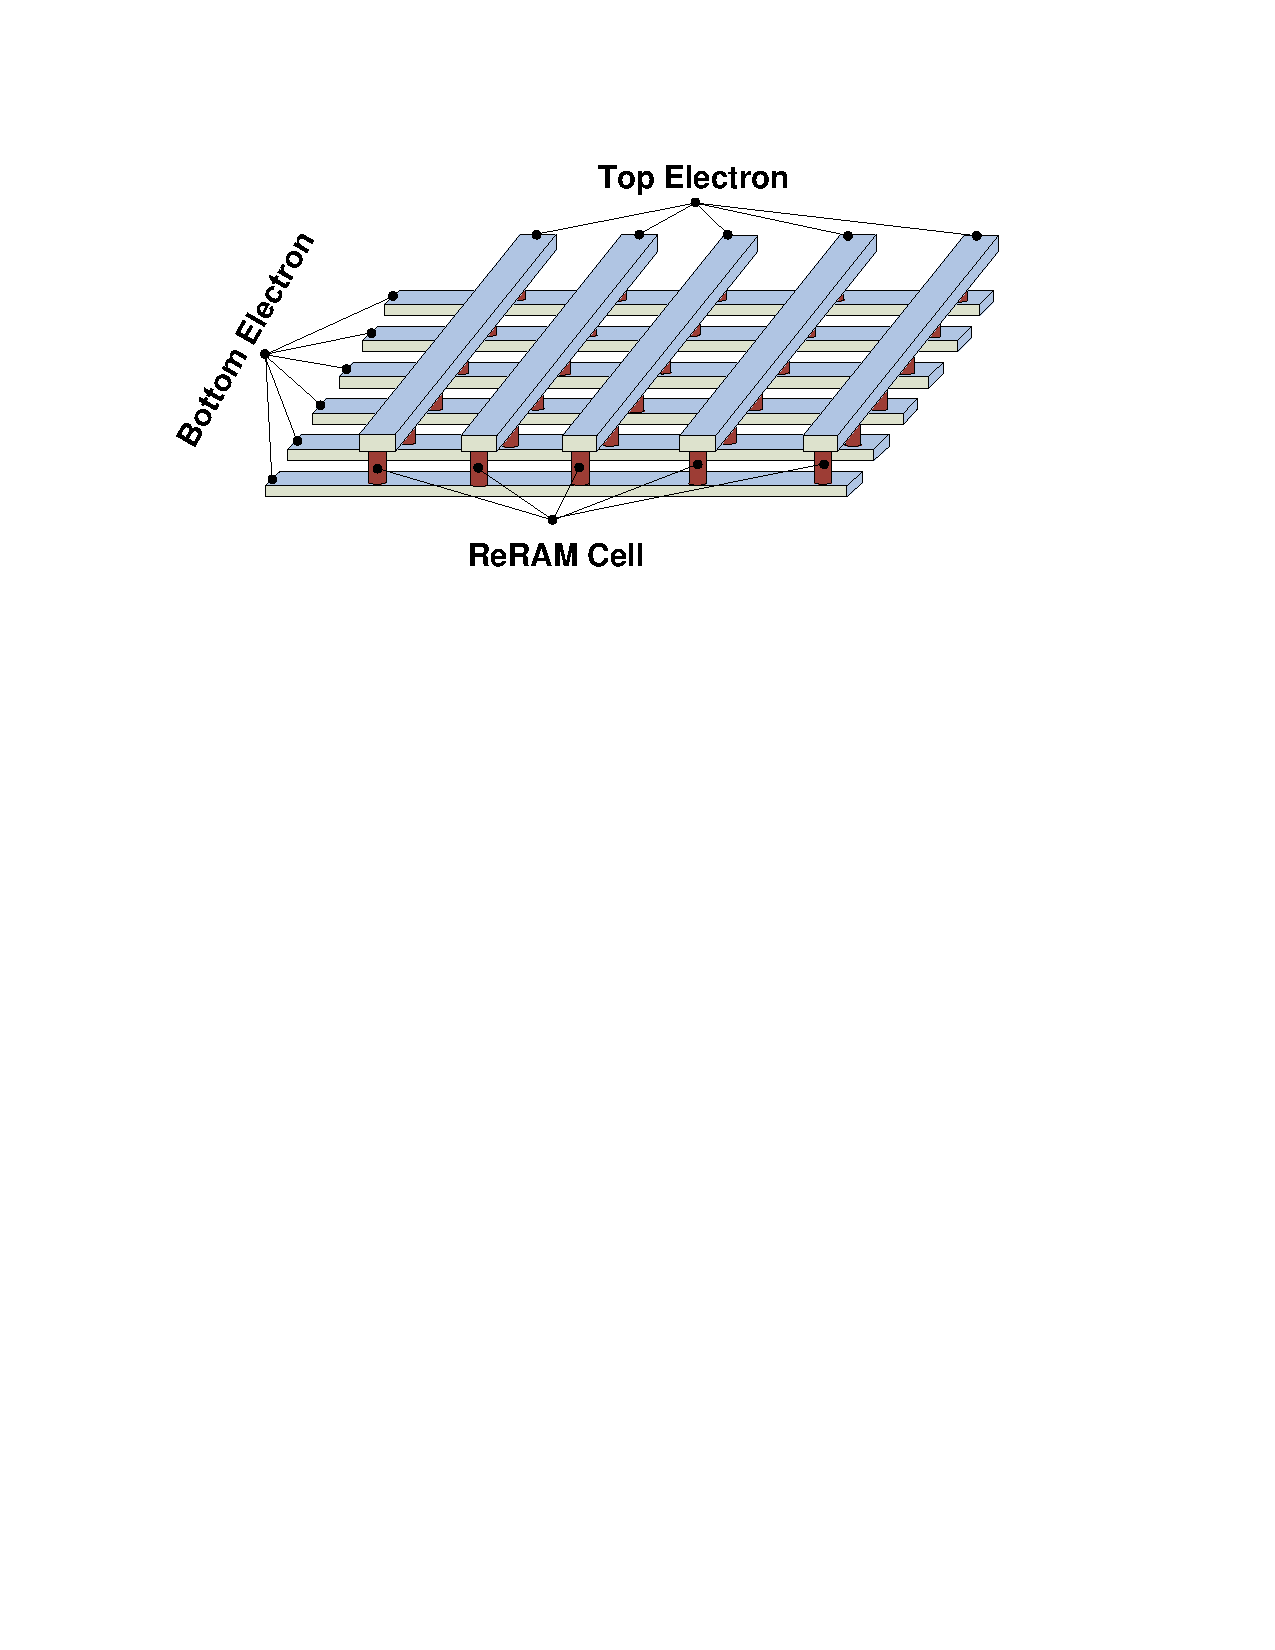
\includegraphics[width=0.45\textwidth]{./figures/crossbar_array.pdf}\\
  \caption{A schematic view of typical cross point architecture.}\label{fig:array}
\end{figure}

\subsection{Motivations}
As aforementioned, although the cross-point structure can provide the fabricate simplicity and area efficiency, it also incur lots of design challenges. Following cases show some examples to demonstrate the disadvantages of the cross-point structure, which motivates the work in this paper.
\begin{enumerate}
  \item \textbf{Reliable Write Operation}\\
  In order to

\begin{figure}
\centering
  % Requires \usepackage{graphicx}
  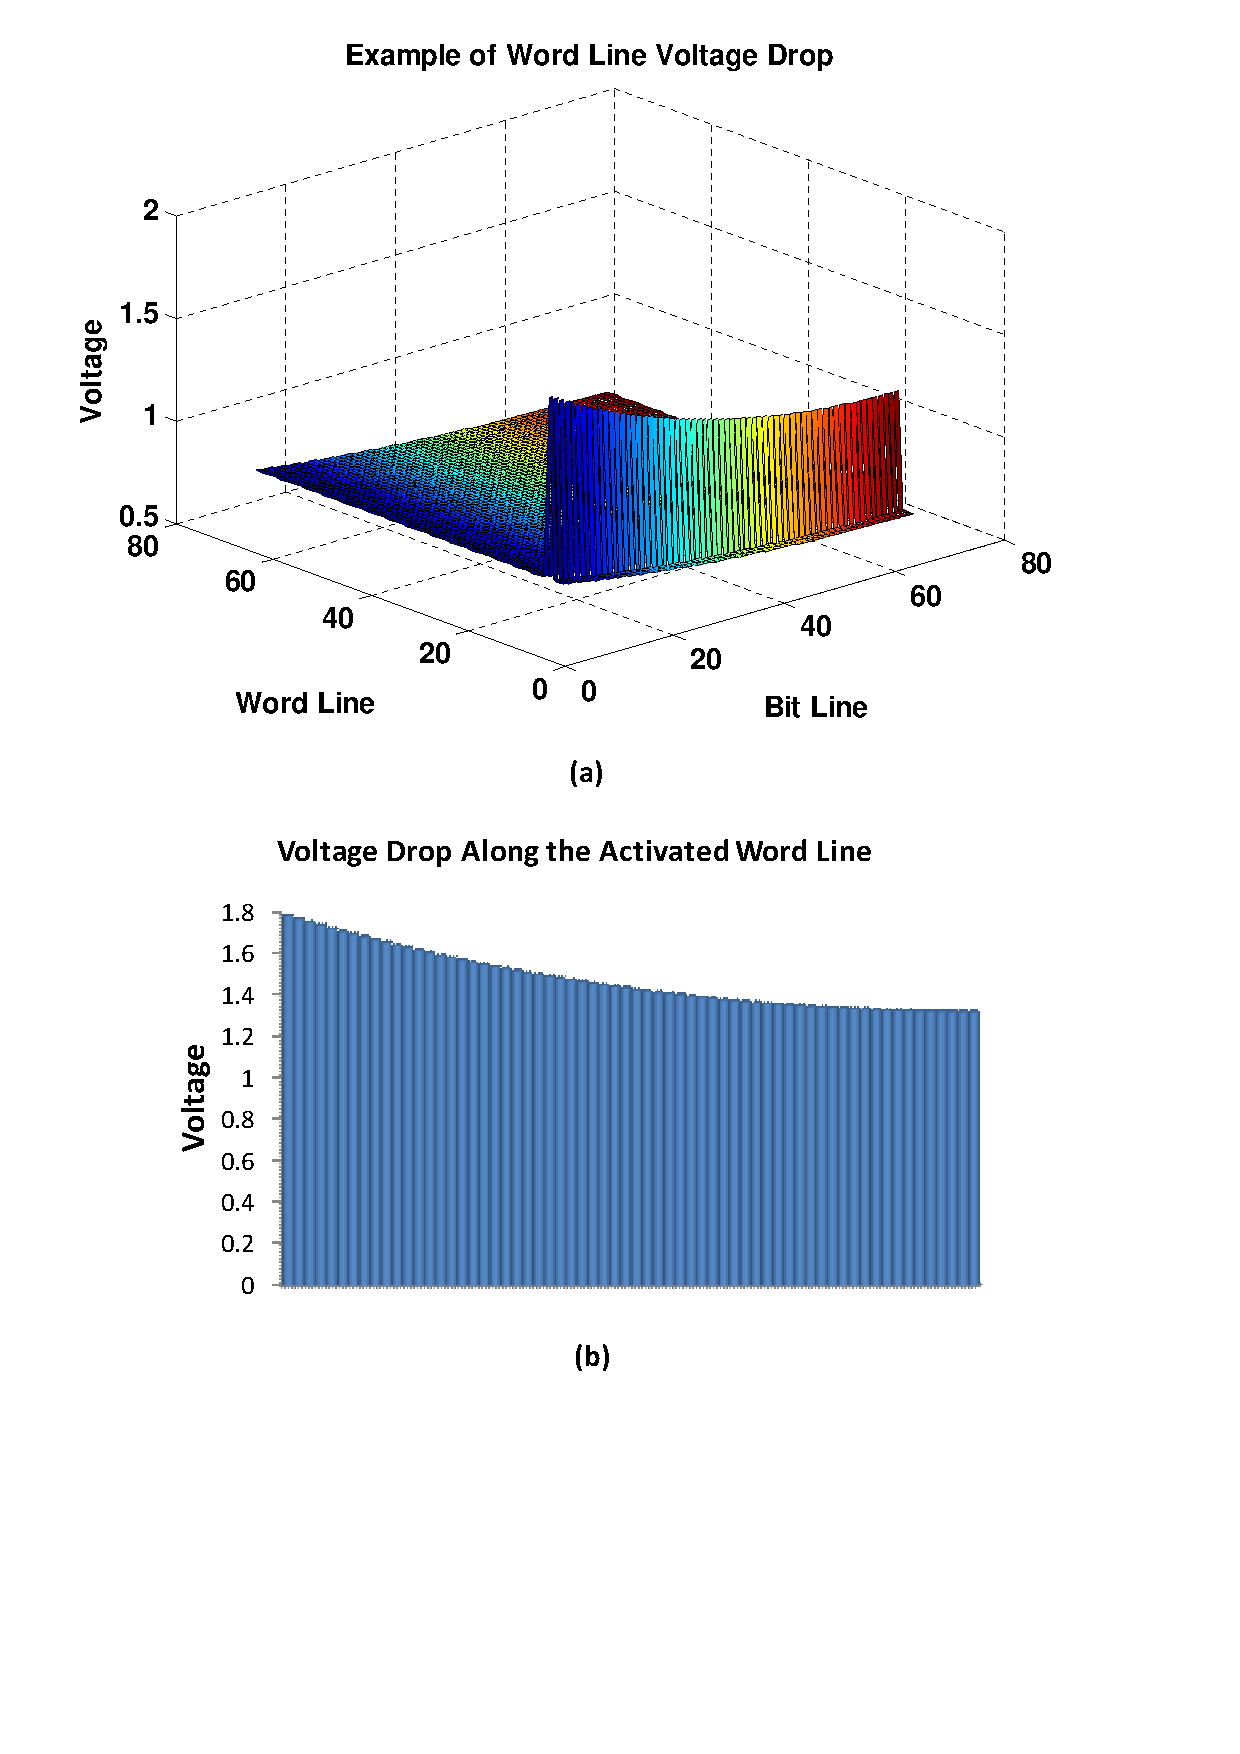
\includegraphics[width=0.4\textwidth]{./figures/example1_large.pdf}\\
  \caption{Case 1: Voltage Drop Along the Word Line during Write Operation.}\label{fig:exampl1}
\end{figure}

  \item \textbf{Read Margin Disturbance}\\
  123
  \item \textbf{Energy Waste Due to Sneak Pass}\\
  123
\end{enumerate}

~\cite{crossbar_NANO08_Nauenheim}~\cite{memristor:analog}~\cite{moore}

